% Options for packages loaded elsewhere
\PassOptionsToPackage{unicode}{hyperref}
\PassOptionsToPackage{hyphens}{url}
%
\documentclass[
]{article}
\usepackage{amsmath,amssymb}
\usepackage{iftex}
\ifPDFTeX
  \usepackage[T1]{fontenc}
  \usepackage[utf8]{inputenc}
  \usepackage{textcomp} % provide euro and other symbols
\else % if luatex or xetex
  \usepackage{unicode-math} % this also loads fontspec
  \defaultfontfeatures{Scale=MatchLowercase}
  \defaultfontfeatures[\rmfamily]{Ligatures=TeX,Scale=1}
\fi
\usepackage{lmodern}
\ifPDFTeX\else
  % xetex/luatex font selection
\fi
% Use upquote if available, for straight quotes in verbatim environments
\IfFileExists{upquote.sty}{\usepackage{upquote}}{}
\IfFileExists{microtype.sty}{% use microtype if available
  \usepackage[]{microtype}
  \UseMicrotypeSet[protrusion]{basicmath} % disable protrusion for tt fonts
}{}
\makeatletter
\@ifundefined{KOMAClassName}{% if non-KOMA class
  \IfFileExists{parskip.sty}{%
    \usepackage{parskip}
  }{% else
    \setlength{\parindent}{0pt}
    \setlength{\parskip}{6pt plus 2pt minus 1pt}}
}{% if KOMA class
  \KOMAoptions{parskip=half}}
\makeatother
\usepackage{xcolor}
\usepackage[margin=1in]{geometry}
\usepackage{color}
\usepackage{fancyvrb}
\newcommand{\VerbBar}{|}
\newcommand{\VERB}{\Verb[commandchars=\\\{\}]}
\DefineVerbatimEnvironment{Highlighting}{Verbatim}{commandchars=\\\{\}}
% Add ',fontsize=\small' for more characters per line
\usepackage{framed}
\definecolor{shadecolor}{RGB}{248,248,248}
\newenvironment{Shaded}{\begin{snugshade}}{\end{snugshade}}
\newcommand{\AlertTok}[1]{\textcolor[rgb]{0.94,0.16,0.16}{#1}}
\newcommand{\AnnotationTok}[1]{\textcolor[rgb]{0.56,0.35,0.01}{\textbf{\textit{#1}}}}
\newcommand{\AttributeTok}[1]{\textcolor[rgb]{0.13,0.29,0.53}{#1}}
\newcommand{\BaseNTok}[1]{\textcolor[rgb]{0.00,0.00,0.81}{#1}}
\newcommand{\BuiltInTok}[1]{#1}
\newcommand{\CharTok}[1]{\textcolor[rgb]{0.31,0.60,0.02}{#1}}
\newcommand{\CommentTok}[1]{\textcolor[rgb]{0.56,0.35,0.01}{\textit{#1}}}
\newcommand{\CommentVarTok}[1]{\textcolor[rgb]{0.56,0.35,0.01}{\textbf{\textit{#1}}}}
\newcommand{\ConstantTok}[1]{\textcolor[rgb]{0.56,0.35,0.01}{#1}}
\newcommand{\ControlFlowTok}[1]{\textcolor[rgb]{0.13,0.29,0.53}{\textbf{#1}}}
\newcommand{\DataTypeTok}[1]{\textcolor[rgb]{0.13,0.29,0.53}{#1}}
\newcommand{\DecValTok}[1]{\textcolor[rgb]{0.00,0.00,0.81}{#1}}
\newcommand{\DocumentationTok}[1]{\textcolor[rgb]{0.56,0.35,0.01}{\textbf{\textit{#1}}}}
\newcommand{\ErrorTok}[1]{\textcolor[rgb]{0.64,0.00,0.00}{\textbf{#1}}}
\newcommand{\ExtensionTok}[1]{#1}
\newcommand{\FloatTok}[1]{\textcolor[rgb]{0.00,0.00,0.81}{#1}}
\newcommand{\FunctionTok}[1]{\textcolor[rgb]{0.13,0.29,0.53}{\textbf{#1}}}
\newcommand{\ImportTok}[1]{#1}
\newcommand{\InformationTok}[1]{\textcolor[rgb]{0.56,0.35,0.01}{\textbf{\textit{#1}}}}
\newcommand{\KeywordTok}[1]{\textcolor[rgb]{0.13,0.29,0.53}{\textbf{#1}}}
\newcommand{\NormalTok}[1]{#1}
\newcommand{\OperatorTok}[1]{\textcolor[rgb]{0.81,0.36,0.00}{\textbf{#1}}}
\newcommand{\OtherTok}[1]{\textcolor[rgb]{0.56,0.35,0.01}{#1}}
\newcommand{\PreprocessorTok}[1]{\textcolor[rgb]{0.56,0.35,0.01}{\textit{#1}}}
\newcommand{\RegionMarkerTok}[1]{#1}
\newcommand{\SpecialCharTok}[1]{\textcolor[rgb]{0.81,0.36,0.00}{\textbf{#1}}}
\newcommand{\SpecialStringTok}[1]{\textcolor[rgb]{0.31,0.60,0.02}{#1}}
\newcommand{\StringTok}[1]{\textcolor[rgb]{0.31,0.60,0.02}{#1}}
\newcommand{\VariableTok}[1]{\textcolor[rgb]{0.00,0.00,0.00}{#1}}
\newcommand{\VerbatimStringTok}[1]{\textcolor[rgb]{0.31,0.60,0.02}{#1}}
\newcommand{\WarningTok}[1]{\textcolor[rgb]{0.56,0.35,0.01}{\textbf{\textit{#1}}}}
\usepackage{graphicx}
\makeatletter
\def\maxwidth{\ifdim\Gin@nat@width>\linewidth\linewidth\else\Gin@nat@width\fi}
\def\maxheight{\ifdim\Gin@nat@height>\textheight\textheight\else\Gin@nat@height\fi}
\makeatother
% Scale images if necessary, so that they will not overflow the page
% margins by default, and it is still possible to overwrite the defaults
% using explicit options in \includegraphics[width, height, ...]{}
\setkeys{Gin}{width=\maxwidth,height=\maxheight,keepaspectratio}
% Set default figure placement to htbp
\makeatletter
\def\fps@figure{htbp}
\makeatother
\setlength{\emergencystretch}{3em} % prevent overfull lines
\providecommand{\tightlist}{%
  \setlength{\itemsep}{0pt}\setlength{\parskip}{0pt}}
\setcounter{secnumdepth}{-\maxdimen} % remove section numbering
\ifLuaTeX
  \usepackage{selnolig}  % disable illegal ligatures
\fi
\IfFileExists{bookmark.sty}{\usepackage{bookmark}}{\usepackage{hyperref}}
\IfFileExists{xurl.sty}{\usepackage{xurl}}{} % add URL line breaks if available
\urlstyle{same}
\hypersetup{
  hidelinks,
  pdfcreator={LaTeX via pandoc}}

\author{}
\date{\vspace{-2.5em}}

\begin{document}

\hypertarget{simple-linear-regression-inference}{%
\section{Simple Linear Regression:
Inference}\label{simple-linear-regression-inference}}

\hypertarget{simple-linear-regression-assumptions}{%
\subsection{Simple Linear Regression
Assumptions}\label{simple-linear-regression-assumptions}}

\begin{itemize}
\item
  Linearity of the relationship between the dependent and independent
  variables
\item
  Independence of the errors (no autocorrelation)
\item
  Constant variance of the errors (homoscedasticity)
\item
  Normality of the error distribution.
\end{itemize}

\hypertarget{simple-linear-regression}{%
\subsection{Simple Linear Regression}\label{simple-linear-regression}}

The simple linear regression model for \(Y\) on \(x\) is
\[Y=\beta_0+\beta_1 x+\epsilon\] where

\(Y\) : the dependent or response variable

\(x\) : the independent or predictor variable, assumed known

\(\beta_0,\beta_1\) : the regression parameters, the intercept and slope
of the regression line

\(\epsilon\) : the random regression error around the line.

\hypertarget{the-simple-linear-regression-equation}{%
\subsection{The simple linear regression
equation}\label{the-simple-linear-regression-equation}}

\begin{itemize}
\tightlist
\item
  The regression equation for a set of \(n\) data points is
  \(\hat{y}=b_0+b_1\;x\), where
  \[b_1=\frac{S_{xy}}{S_{xx}}=\frac{\sum (x_i-\bar{x})(y_i-\bar{y})}{\sum (x_i-\bar{x})^2}\]
  and \[b_0=\bar{y}-b_1\; \bar{x}\]
\item
  \(y\) is the dependent variable (or response variable) and \(x\) is
  the independent variable (predictor variable or explanatory variable).
\item
  \(b_0\) is called the \textbf{y-intercept} and \(b_1\) is called the
  \textbf{slope}.
\end{itemize}

\hypertarget{residual-standard-error-s_e}{%
\subsection{\texorpdfstring{Residual standard error,
\(s_e\)}{Residual standard error, s\_e}}\label{residual-standard-error-s_e}}

The residual standard error, \(s_e\), is defined by
\[s_e=\sqrt{\frac{SSE}{n-2}}\] where \(SSE\) is the error sum of squares
(also known as the residual sum of squares, RSS) which can be defined as
\[SSE=\sum e^2_i=\sum(y_i-\hat{y}_i)^2=S_{yy}-\frac{S^2_{xy}}{S_{xx}}\]
\(s_e\) indicates how much, on average, the observed values of the
response variable differ from the predicated values of the response
variable. Under the simple linear regression assumptions, \(s_e\) is an
unbiased estimate for the error standard deviation \(\sigma\).

\hypertarget{properties-of-regression-coefficients}{%
\subsection{Properties of Regression
Coefficients}\label{properties-of-regression-coefficients}}

Under the simple linear regression assumptions, the least square
estimates \(b_0\) and \(b_1\) are unbiased for the \(\beta_0\) and
\(\beta_1\), respectively, i.e.

\(E[b_0]=\beta_0\) and \(E[b_1]=\beta_1\).

The variances of the least squares estimators in simple linear
regression are:

\[Var[b_0]=\sigma^2_{b_0}=\sigma^2\left(\frac{1}{n}+\frac{\bar{x}^2}{S_{xx}}\right)\]

\[Var[b_1]=\sigma^2_{b_1}=\frac{\sigma^2}{S_{xx}}\]
\[Cov[b_0,b_1]=\sigma_{b_0,b_1}=-\sigma^2\frac{\bar{x}}{S_{xx}}\]

We use \(s_e\) to estimate the error standard deviation \(\sigma\):

\[s^2_{b_0}=s_e^2\left(\frac{1}{n}+\frac{\bar{x}^2}{S_{xx}}\right)\]

\[s^2_{b_1}=\frac{s_e^2}{S_{xx}}\]

\[s_{b_0,b_1}=-s_e^2\frac{\bar{x}}{S_{xx}}\]

\hypertarget{sampling-distribution-of-the-least-square-estimators}{%
\subsection{Sampling distribution of the least square
estimators}\label{sampling-distribution-of-the-least-square-estimators}}

For the Normal error simple linear regression model:
\[b_0\sim N(\beta_0,\sigma^2_{b_0}) \rightarrow 
\frac{b_0-\beta_0}{\sigma_{b_0}}\sim N(0,1)\] and
\[b_1\sim N(\beta_1,\sigma^2_{b_1}) \rightarrow
\frac{b_1-\beta_1}{\sigma_{b_1}}\sim N(0,1)\]

We use \(s_e\) to estimate the error standard deviation \(\sigma\):
\[\frac{b_0-\beta_0}{s_{b_0}}\sim t_{n-2}\] and
\[\frac{b_1-\beta_1}{s_{b_1}}\sim t_{n-2}\]

\hypertarget{degrees-of-freedom}{%
\subsection{Degrees of Freedom}\label{degrees-of-freedom}}

\begin{itemize}
\item
  In statistics, degrees of freedom are the number of independent pieces
  of information that go into the estimate of a particular parameter.
\item
  Typically, the degrees of freedom of an estimate of a parameter are
  equal to the number of independent observations that go into the
  estimate, minus the number of parameters that are estimated as
  intermediate steps in the estimation of the parameter itself.
\item
  The sample variance has \(n - 1\) degrees of freedom, since it is
  computed from n pieces of data, minus the 1 parameter estimated as
  intermediate step, the sample mean. Similarly, having estimated the
  sample mean we only have \(n - 1\) independent pieces of data left, as
  if we are given the sample mean and any \(n - 1\) of the observations
  then we can determine the value of remaining observation exactly.
\end{itemize}

\[s^2=\frac{\sum(x_i-\bar{x})^2}{n-1}\]

\begin{itemize}
\tightlist
\item
  In linear regression, the degrees of freedom of the residuals is
  \(df=n-k^*\), where \(k^*\) is the numbers of estimated parameters
  (including the intercept). So for the simple linear regression, we are
  estimating \(\beta_0\) and \(\beta_1\), thus \(df=n-2\).
\end{itemize}

\hypertarget{inference-for-the-intercept-beta_0}{%
\subsection{\texorpdfstring{Inference for the intercept
\(\beta_0\)}{Inference for the intercept \textbackslash beta\_0}}\label{inference-for-the-intercept-beta_0}}

\begin{itemize}
\item
  Hypotheses:\[H_0:\beta_0=0\;\; \text{against}\;\; H_1:\beta_0\neq 0\]
\item
  Test statistic: \[t=\frac{b_0}{s_{b_0}}\] has a t-distribution with
  \(df=n-2\), where \(s_{b_0}\) is the standard error of \(b_0\), and
  given by \[s_{b_0}=s_e\sqrt{\frac{1}{n}+\frac{\bar{x}^2}{S_{xx}}}\]
  and
\end{itemize}

\[s_e=\sqrt{\frac{SSE}{n-2}}=\sqrt{\frac{\sum(y_i-\hat{y}_i)^2}{n-2}}\]
We reject \(H_0\) at level \(\alpha\) if \(|t|>t_{\alpha/2}\) with
\(df=n-2\).

\begin{itemize}
\tightlist
\item
  100(1-\(\alpha\))\% confidence interval for \(\beta_0\),
\end{itemize}

\[b_0 \pm t_{\alpha/2} .\;s_{b_0}\] where \(t_{\alpha/2}\) is critical
value obtained from the t‐distribution table with \(df=n-2\).

\hypertarget{inference-for-the-slope-beta_1}{%
\subsection{\texorpdfstring{Inference for the slope
\(\beta_1\)}{Inference for the slope \textbackslash beta\_1}}\label{inference-for-the-slope-beta_1}}

\begin{itemize}
\item
  Hypotheses: \[H_0:\beta_1=0\;\; \text{against}\;\; H_1:\beta_1\neq 0\]
\item
  Test statistic: \[t=\frac{b_1}{s_{b_1}}\] has a t-distribution with
  \(df=n-2\), where \(s_{b_1}\) is the standard error of \(b_1\),and
  given by
\end{itemize}

\[s_{b_1}=\frac{s_e}{\sqrt{S_{xx}}}\]

and

\[s_e=\sqrt{\frac{SSE}{n-2}}=\sqrt{\frac{\sum(y_i-\hat{y}_i)^2}{n-2}}\]
We reject \(H_0\) at level \(\alpha\) if \(|t|>t_{\alpha/2}\) with
\(df=n-2\).

\begin{itemize}
\tightlist
\item
  100(1-\(\alpha\))\% confidence interval for \(\beta_1\),
\end{itemize}

\[b_1 \pm t_{\alpha/2} \;s_{b_1}\] where \(t_{\alpha/2}\) is critical
value obtained from the t‐distribution table with \(df=n-2\).

\begin{center}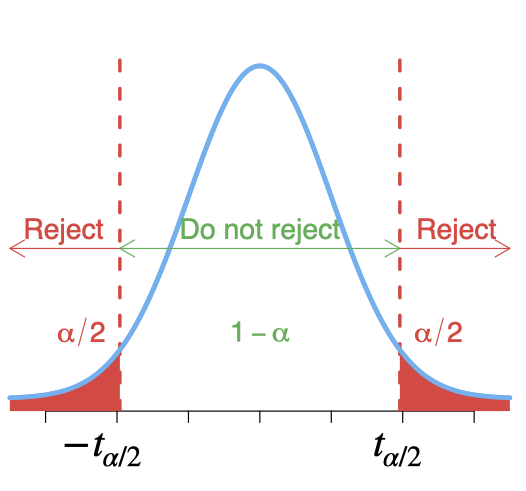
\includegraphics[width=0.3\linewidth,height=0.3\textheight]{figures/Ttest2} \end{center}

\hypertarget{how-useful-is-the-regression-model}{%
\subsection{How useful is the regression
model?}\label{how-useful-is-the-regression-model}}

\textbf{Goodness of fit test}

\begin{itemize}
\item
  We test the null hypothesis \(H_0:\beta_1=0\) against
  \(H_1:\beta_1\neq 0\), the F-statistic
  \[F=\frac{MSR}{MSE}=\frac{SSR}{SSE/(n-2)}\] has F-distribution with
  degrees of freedom \(df_1=1\) and \(df_2=n-2\).
\item
  We reject \(H_0\), at level \(\alpha\), if
  \(F>F_{\alpha}(df_1,df_2)\).
\item
  For a simple linear regression ONLY, F-test is equivalent to t-test
  for \(\beta_1\).
\end{itemize}

\begin{center}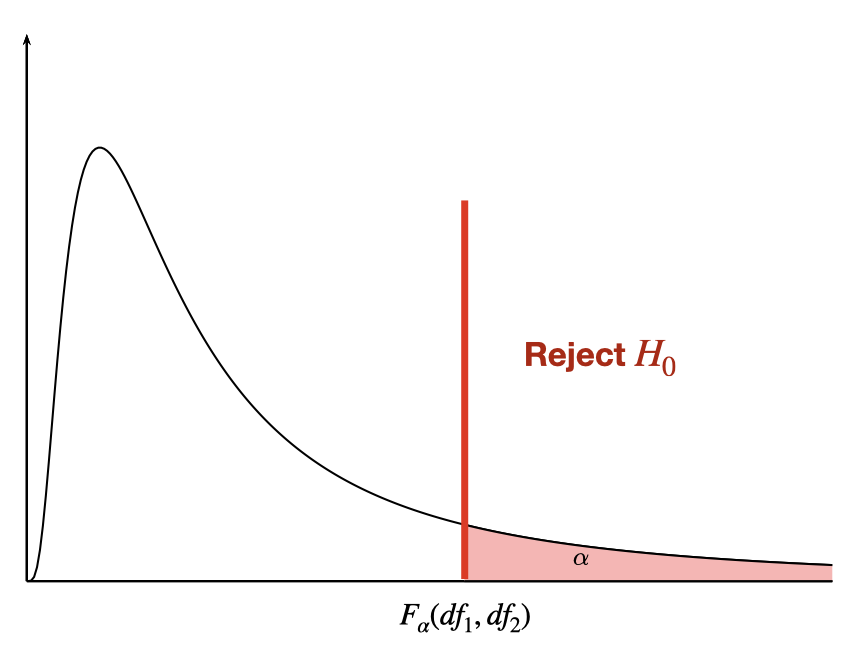
\includegraphics[width=0.4\linewidth,height=0.4\textheight]{figures/Ftest} \end{center}

\hypertarget{example-used-cars-cont.}{%
\subsection{Example: used cars (cont.)}\label{example-used-cars-cont.}}

\begin{Shaded}
\begin{Highlighting}[]
\NormalTok{Price}\OtherTok{\textless{}{-}}\FunctionTok{c}\NormalTok{(}\DecValTok{85}\NormalTok{, }\DecValTok{103}\NormalTok{,  }\DecValTok{70}\NormalTok{,  }\DecValTok{82}\NormalTok{,  }\DecValTok{89}\NormalTok{,  }\DecValTok{98}\NormalTok{,  }\DecValTok{66}\NormalTok{,  }\DecValTok{95}\NormalTok{, }\DecValTok{169}\NormalTok{,  }\DecValTok{70}\NormalTok{,  }\DecValTok{48}\NormalTok{)}
\NormalTok{Age}\OtherTok{\textless{}{-}} \FunctionTok{c}\NormalTok{(}\DecValTok{5}\NormalTok{, }\DecValTok{4}\NormalTok{, }\DecValTok{6}\NormalTok{, }\DecValTok{5}\NormalTok{, }\DecValTok{5}\NormalTok{, }\DecValTok{5}\NormalTok{, }\DecValTok{6}\NormalTok{, }\DecValTok{6}\NormalTok{, }\DecValTok{2}\NormalTok{, }\DecValTok{7}\NormalTok{, }\DecValTok{7}\NormalTok{)}
\NormalTok{carSales}\OtherTok{\textless{}{-}}\FunctionTok{data.frame}\NormalTok{(Price,Age)}
\FunctionTok{str}\NormalTok{(carSales)}
\end{Highlighting}
\end{Shaded}

\begin{verbatim}
## 'data.frame':    11 obs. of  2 variables:
##  $ Price: num  85 103 70 82 89 98 66 95 169 70 ...
##  $ Age  : num  5 4 6 5 5 5 6 6 2 7 ...
\end{verbatim}

\begin{Shaded}
\begin{Highlighting}[]
\CommentTok{\# simple linear regression}
\NormalTok{reg}\OtherTok{\textless{}{-}}\FunctionTok{lm}\NormalTok{(Price}\SpecialCharTok{\textasciitilde{}}\NormalTok{Age)}
\FunctionTok{summary}\NormalTok{(reg)}
\end{Highlighting}
\end{Shaded}

\begin{verbatim}
## 
## Call:
## lm(formula = Price ~ Age)
## 
## Residuals:
##     Min      1Q  Median      3Q     Max 
## -12.162  -8.531  -5.162   8.946  21.099 
## 
## Coefficients:
##             Estimate Std. Error t value Pr(>|t|)    
## (Intercept)   195.47      15.24  12.826 4.36e-07 ***
## Age           -20.26       2.80  -7.237 4.88e-05 ***
## ---
## Signif. codes:  0 '***' 0.001 '**' 0.01 '*' 0.05 '.' 0.1 ' ' 1
## 
## Residual standard error: 12.58 on 9 degrees of freedom
## Multiple R-squared:  0.8534, Adjusted R-squared:  0.8371 
## F-statistic: 52.38 on 1 and 9 DF,  p-value: 4.882e-05
\end{verbatim}

\(~\)

\begin{Shaded}
\begin{Highlighting}[]
\CommentTok{\# To obtain the confidence intervals }
\FunctionTok{confint}\NormalTok{(reg, }\AttributeTok{level=}\FloatTok{0.95}\NormalTok{)}
\end{Highlighting}
\end{Shaded}

\begin{verbatim}
##                 2.5 %    97.5 %
## (Intercept) 160.99243 229.94451
## Age         -26.59419 -13.92833
\end{verbatim}

\hypertarget{r-output}{%
\subsection{R output}\label{r-output}}

\begin{center}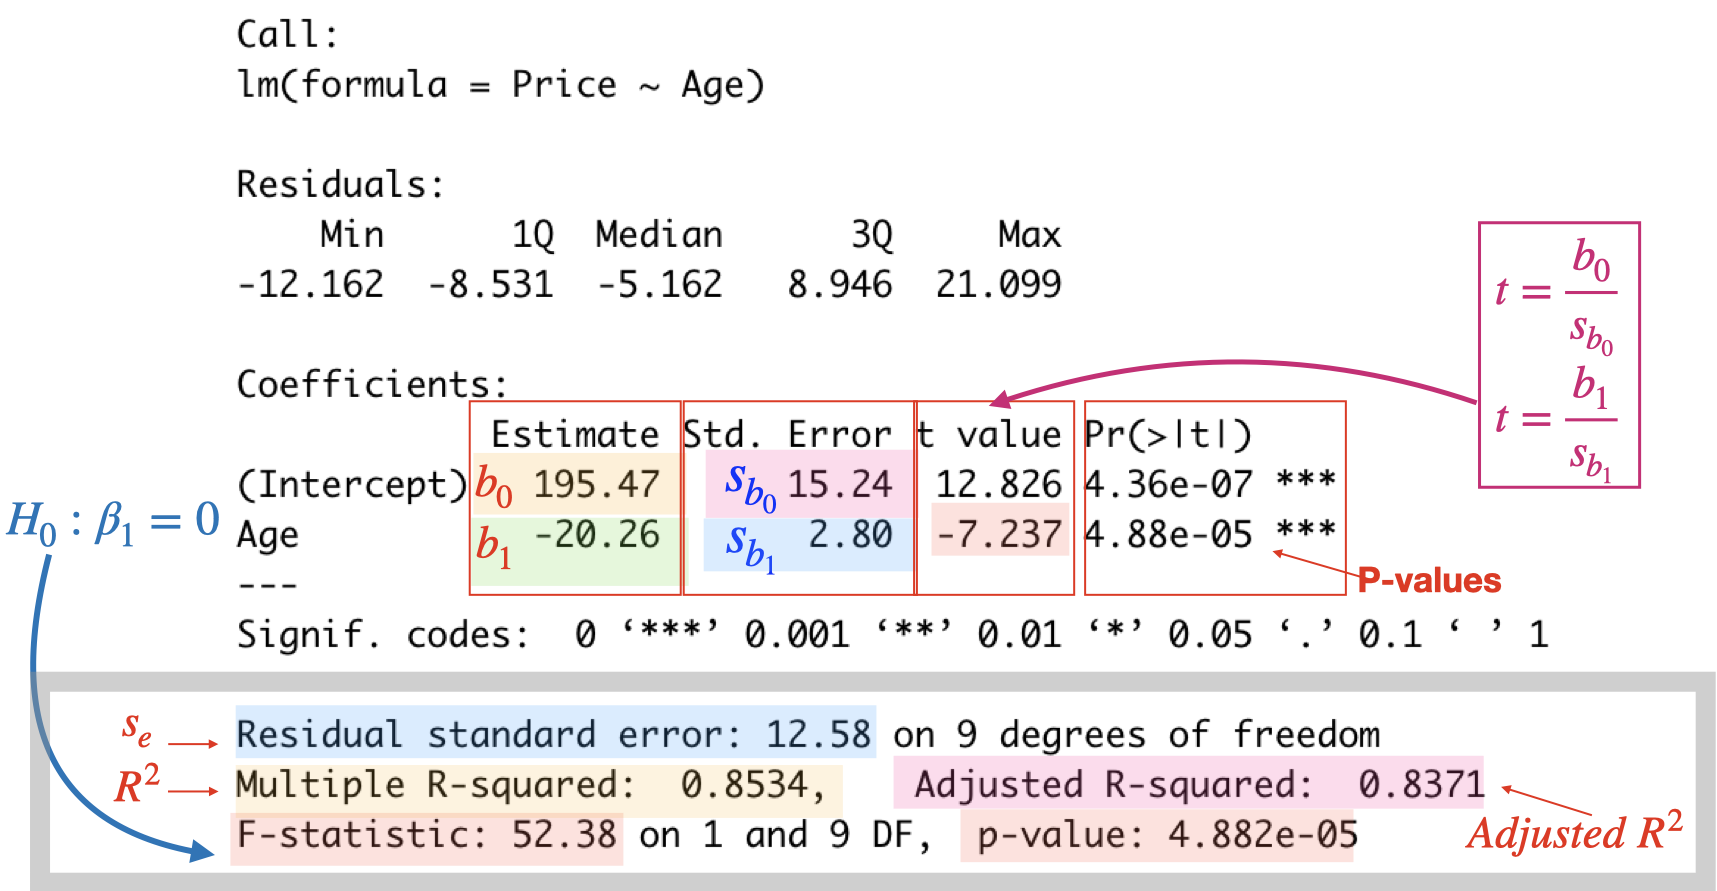
\includegraphics[width=0.8\linewidth,height=0.8\textheight]{figures/regRoutput} \end{center}

\end{document}
